夏天时忽略上方房间地暖的影响,同时将$T_next = 26.8℃$代入\eqref{boundary},使用Matlab进行仿真,房间的温度分布如下图所示:
\\
\begin{figure}[h]
    \centering
    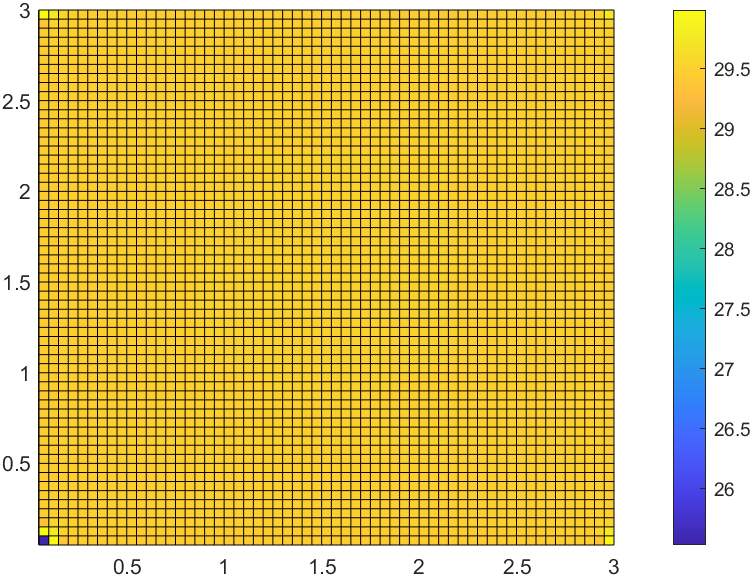
\includegraphics[width = 5.5cm]{figures/mainroom-summer.png}
    \caption{夏天非采暖房间温度分布}
    \label{夏天非采暖房间温度分布}
\end{figure}

夏天非采暖房间的平均温度为29℃。

在进行仿真时,由于夏天房间墙壁上的热流方向与冬天房间墙壁相反,因此需要调整室内传热和墙壁导热的计算顺序,否则会出现结果不准确的现象。